\documentclass[a4paper,11pt,notitlepage]{report}

\usepackage{graphicx}
\usepackage[utf8]{inputenc}
\usepackage[T1]{fontenc}
\usepackage[ngerman]{babel}
\usepackage{bibgerm}
\usepackage{amsmath,amssymb,amsthm}
\usepackage{color}
\usepackage{enumerate}
\usepackage{tabularx}
\usepackage{subfig}
\usepackage{fancyhdr}
\usepackage{upgreek}
\usepackage[pdftex,pdfpagelabels,colorlinks,backref,pagebackref]{hyperref}
\usepackage{tikz} % SELBST HINZUGEFÜGT
\usepackage{graphicx}
\usepackage{framed}
\usepackage{lmodern}
% == Set the heading style ===================================================
\setlength{\headheight}{14pt}
\pagestyle{fancyplain}
\renewcommand{\chaptermark}[1]{\markboth{#1}{}}
\renewcommand{\sectionmark}[1]{\markright{\thesection\ #1}}
\lhead[\fancyplain{}{\thepage}]{\fancyplain{}{\rightmark}}
\rhead[\fancyplain{}{\leftmark}]{\fancyplain{}{\thepage}}
\cfoot{}
\renewcommand{\headrulewidth}{0.4pt}
% ============================================================================

% == Set correct values for fitting floats ===================================
\tolerance=2000
\emergencystretch=10pt

\setcounter{topnumber}{3}
\setcounter{totalnumber}{5}
\setcounter{bottomnumber}{2}

% To make those darn floats fit where they should
\setcounter{totalnumber}{9}
\setcounter{topnumber}{9}
\setcounter{bottomnumber}{9}
\renewcommand{\textfraction}{0.00}
\renewcommand{\topfraction}{1.0}
\renewcommand{\bottomfraction}{1.0}
% ============================================================================

% == German definitions for theorems etc. ==================================== 
\newtheorem{definition}{Definition}[chapter]
\newtheorem{theorem}{Satz}[chapter]
\newtheorem{lemma}{Lemma}[chapter]
\newtheorem{proposition}{Proposition}[chapter]
\newtheorem{corollary}{Korollar}[chapter]
\newtheorem{observation}{Beobachtung}[chapter]
\newtheorem{fact}{Fakt}[chapter]
\newtheorem{remark}{Bemerkung}[chapter]
\newtheorem{example}{Beispiel}[chapter]
% ============================================================================

% == Abkürzungen für die reellen, natürlichen, ganzen,... Zahlen =============
\newcommand{\R}{{\ensuremath{\mathbb{R}}}}
\newcommand{\N}{{\ensuremath{\mathbb{N}}}}
\newcommand{\Z}{{\ensuremath{\mathbb{Z}}}}
\newcommand{\C}{{\ensuremath{\mathbb{C}}}}
\newcommand{\Q}{{\ensuremath{\mathbb{Q}}}}
\newcommand{\F}{{\ensuremath{\mathbb{F}}}}
\newcommand{\Prim}{{\ensuremath{\mathbb{P}}}}
% ============================================================================

% == Makros für Autorenname und -adresse =====================================
\newcommand{\myaddress}[6]{%
  \parbox{\textwidth}{\textbf{\large #1}\\
    #2\\ #3\\ #4\\ 
    \ifthenelse{\equal{#5}{}}{}{Email: \href{mailto:#5}{\texttt{#5}}\\}
    \ifthenelse{\equal{#6}{}}{}{WWW: \href{#6}{\path|#6|}\\}
  } 
}

\newcommand{\myauthor}[1]{%
  \addtocontents{toc}{\protect\hspace{3.35ex}%
  \textsl{#1}\par}\vspace{-4ex}\quad\hfill\textsl{\Large #1}\vspace{8ex}}

\newcommand{\myname}[1]{\Large #1}

%%%%%%%%%%%%%%%%%%%%%%%%%%%%%%%%%%%%%%%%%%%%%%%%%%
% Tragen Sie in der folg. Zeile Ihren Namen ein: %
%%%%%%%%%%%%%%%%%%%%%%%%%%%%%%%%%%%%%%%%%%%%%%%%%%

\newcommand{\OO}{{\ensuremath{\mathcal{O}}}}

\renewcommand{\thechapter}{\Roman{chapter}}
\renewcommand{\thesection}{\arabic{section}}


\newenvironment{Kasten}[1]
{
\hspace{0.05\linewidth}
\begin{center}
\begin{minipage}{0.9\linewidth}
\setlength{\fboxsep}{10pt}
%\setlength{\fboxsep}{18pt}
%\definecolor{shadecolor}{gray}{0.9}
\definecolor{shadecolor}{gray}{1}
\definecolor{framecolor}{gray}{0}
\def\FrameCommand{\fcolorbox{framecolor}{shadecolor}}
\MakeFramed {\FrameRestore}
\subsection{#1}
\begin{itshape}
}
{
\end{itshape}
\endMakeFramed
\end{minipage}
\end{center}
%\vspace{1em}
}

\begin{document}
\shorthandoff{"}
\setcounter{chapter}{0}

\begin{titlepage}
	\begin{center}	
		\LARGE \textbf{{Einführung in die Geometrie und Topologie - Mitschrieb -} \\[5ex] 
    		{\Large Vorlesung im Wintersemester 2011/2012\\[5ex]}}
	\end{center}
	\begin{center}
		\Large Sarah Lutteropp, Simon Bischof
	\end{center}
	\begin{center}
		\today
	\end{center}
	\vspace{2cm}
	\begin{center}
		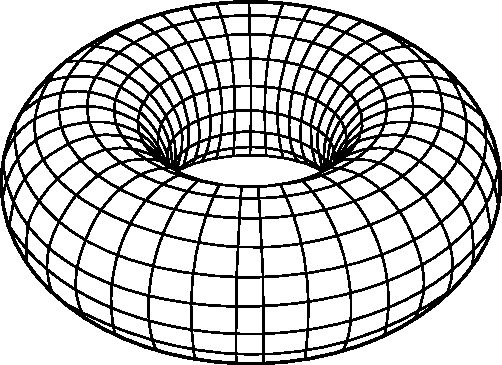
\includegraphics[width=0.8\textwidth]{torus2.pdf}
	\end{center}
\end{titlepage}
%\maketitle
\setcounter{tocdepth}{1}
\tableofcontents

\section*{Zusammenfassung}
Dies ist ein Mitschrieb der Vorlesung “Einführung in die Geometrie und Topologie” vom Wintersemester 2011/2012 am Karlsruher Institut für Technologie, die von Herrn Prof. Dr. Wilderich Tuschmann gehalten wird.

\chapter{Homotopie und Fundamentalgruppe}
\setcounter{section}{-1}
\section{Vorwort}
\begin{Kasten}{Topologischer Raum}
Ein \underline{topologischer Raum} $X$ ist gegeben durch eine Menge $X$ und ein System $\OO$ von Teilmengen von $X$, den so genannten \underline{offenen Mengen} von $X$, welches unter beliebigen Vereinigungen und endlichen Durchschnitten abgeschlossen ist und $X$ und die leere Menge $\emptyset$ als Elemente enthält.
\newline
$X$ Menge, $\OO \subset \mathcal{P}(X) \colon$
\begin{enumerate}[(1)]
	\item $O_1, O_2 \in \OO \Rightarrow O_1 \cap O_2 \in \OO$
	\item $O_\alpha \in \OO, \alpha \in A, A \text{ Indexmenge} \Rightarrow \bigcup\limits_{\alpha \in A}{O_\alpha} \in \OO$
	\item $X, \emptyset \in \OO$
\end{enumerate}
\end{Kasten}

\begin{example}
\OO = $\{X, \emptyset\} \Rightarrow (X,\OO)$ ist topologischer Raum!
\end{example}

\begin{example}
$$X \text{ Menge, }\OO = \left\{\{x\} \mid x\in X\right\} + \text{Axiome, die zu erfüllen sind} \leadsto \tilde{\OO} = \mathcal{P}(X)$$
$\Rightarrow (X,\tilde{\OO})$ ist topologischer Raum.
$\OO$ ist "Basis" der Topologie $\tilde{\OO}$.
\end{example}

\begin{Kasten}{Metrischer Raum}
Ein \underline{metrischer Raum} $X$ ist eine Menge $X$ mit einer Abbildung $d \colon X \times X \rightarrow \R$, der \underline{"Metrik"} auf $X$, die folgende Eigenschaften erfüllt:
$\forall x,y,z \in X$
\begin{enumerate}[(1)]
	\item $d(x,y) = d(y,x)$ \underline{"Symmetrie"}
	\item $d(x,y) = 0 \Leftrightarrow x = y, d(x,y) \geq 0$ \underline{"Definitheit"}
	\item $d(x,z) \leq d(x,y) + d(y,z)$ \underline{"Dreiecksungleichung"}
\end{enumerate}
\end{Kasten}

%\begin{Kasten}[stetig]
\begin{Kasten}{Stetigkeit}
Eine Abbildung $F \colon X \rightarrow Y$ zwischen topologischen Räumen $X$ und $Y$ heißt \underline{stetig}, falls die F-Urbilder offener Mengen in $Y$ offene Teilmengen von $X$ sind.
%\end{Kasten}
\end{Kasten}

\begin{figure}[h]
\centering
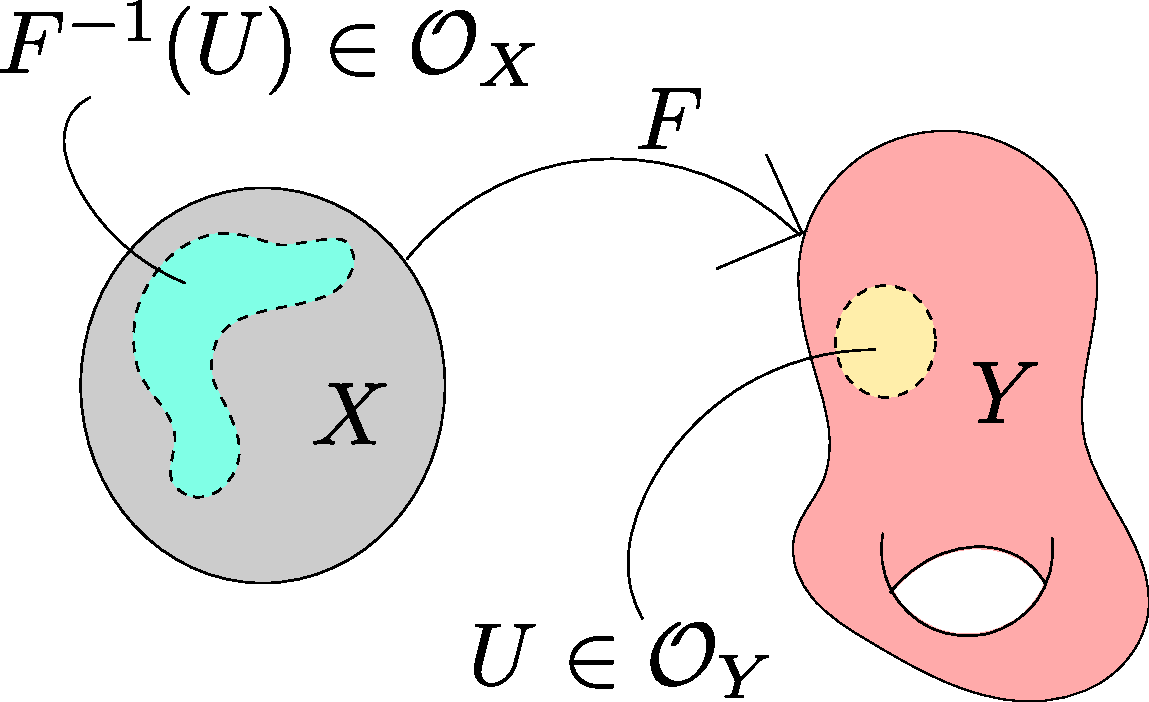
\includegraphics[width=0.8\textwidth]{images/stetigeAbb.pdf}
\caption{Stetige Abbildung}
\end{figure}

\begin{remark}
Ist $(X,d)$ ein metrischer Raum, so sind die offenen Mengen der von der Metrik induzierten Topologie Vereinigungen von endlichen Durchschnitten von Umgebungen
$U_{\epsilon}(x):=\{y \in X \mid d (x,y) < \epsilon \} (\epsilon > 0)$, 
und $F \colon (X,d) \rightarrow (Y,d')$ ist stetig im obigen Sinn genau dann, falls für alle $\epsilon > 0$ ein $\delta > 0$ existiert mit $F(U_\delta (x)) \subset U_\epsilon (F(x))$.
\end{remark}

%\begin{Kasten}[Homotopie]
\begin{Kasten}{Homotopie}
Eine \underline{Homotopie} $H \colon f \simeq g$ zwischen zwei (stetigen) Abbildungen $f,g \colon X \rightarrow Y$ ist eine (stetige) Abbildung $$H \colon X \times I \footnote{$I = [0,1] \subset \R$} \rightarrow Y, (x,t) \mapsto H(x,t)$$ mit $H(x,0) = f(x) \text{ und } H(x,1) = g(x) \forall x \in X$.
%\end{Kasten}
\end{Kasten}


\begin{figure}[h]
\centering
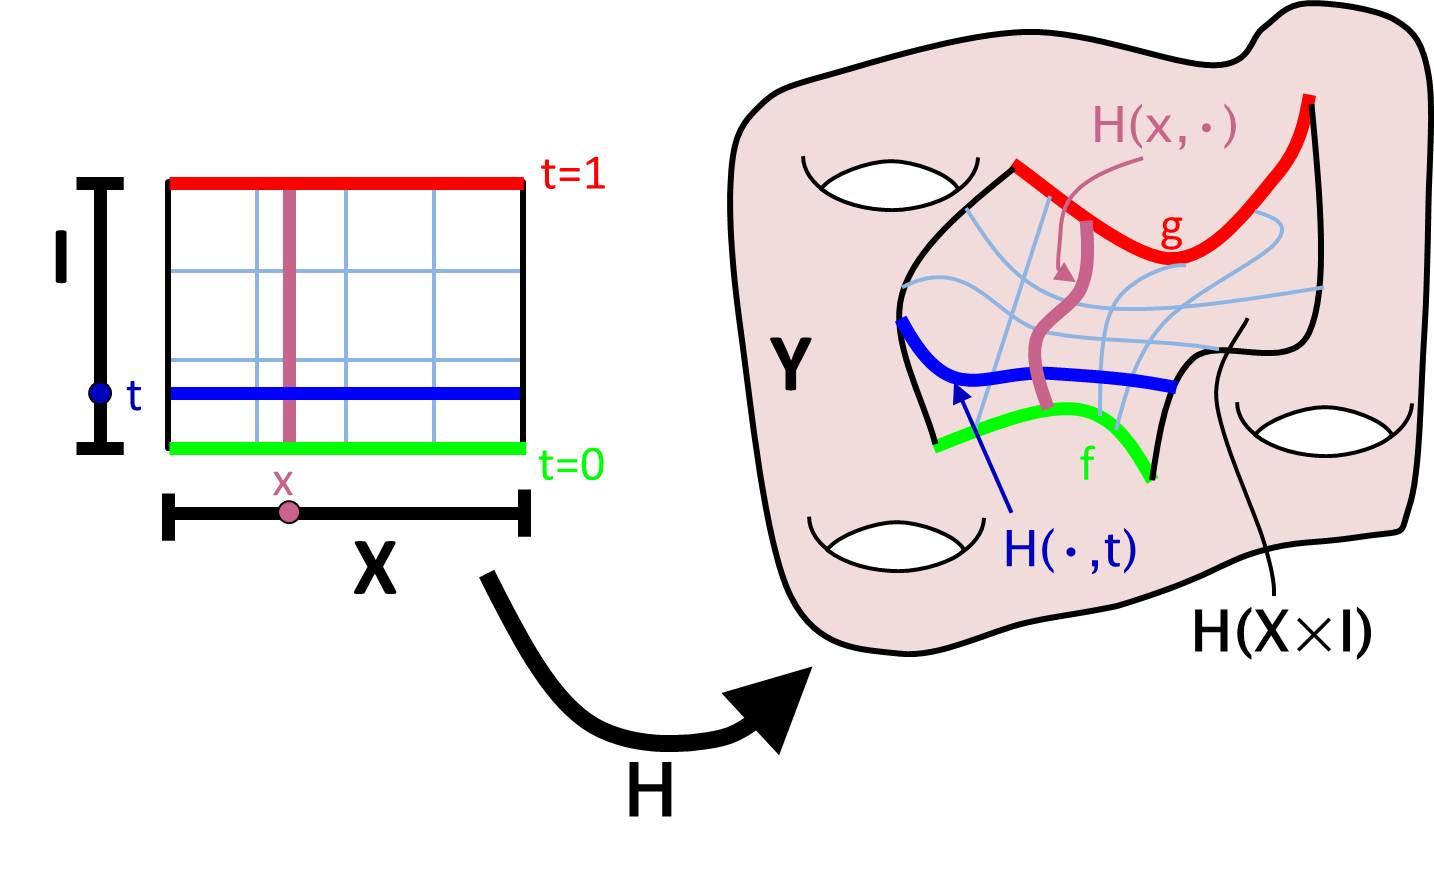
\includegraphics[width=0.7\textwidth]{images/Homotopie.jpg}
\caption{Homotopie}
\end{figure}

\begin{figure}[h]
\centering
\subfloat{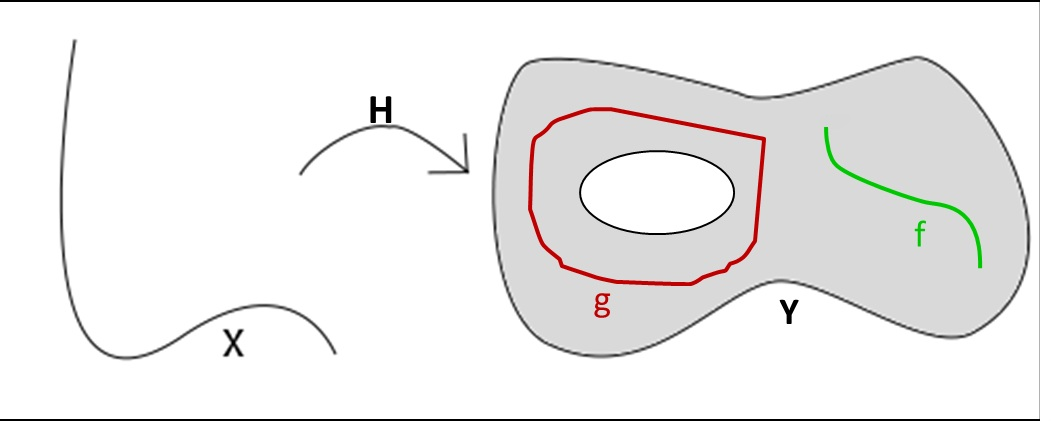
\includegraphics[width=0.5\textwidth]{images/nicht_homotop_1.jpg}}\qquad
\subfloat{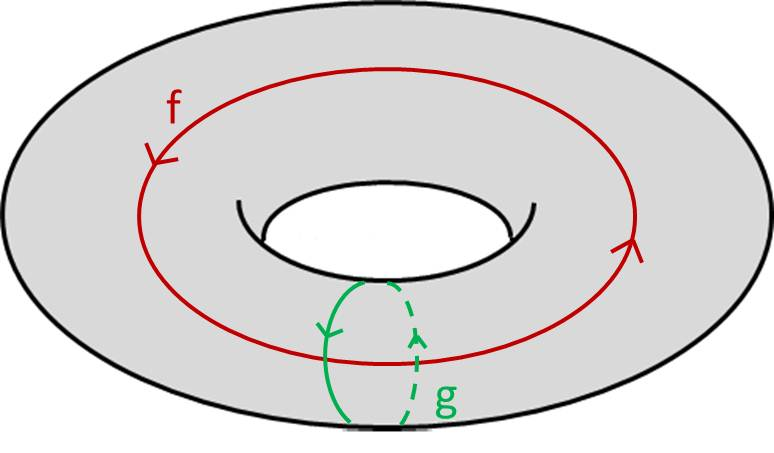
\includegraphics[width=0.4\textwidth]{images/nicht_homotop_2.jpg}}
\caption{f und g sind jeweils \underline{nicht} homotop!}
\end{figure}

\begin{remark}
$H$ heißt auch \underline{Homotopie} \underline{\underline{von $f$ nach $g$}}, eine solche ist also eine parametrisierte Schar von Abbildungen mit "Anfang" $f$ und "Ende" $g$. $f$ und $g$ heißen dann \underline{homotop}, in Zeichen: $f \simeq g$.
\end{remark}

\paragraph{Erinnerung}
Sind $X$ und $Y$ topologische Räume, so ist eine Homotopie $H = (h_t), t \in [0,1]$, eine parametrisierte Schar von stetigen Abbildungen $h_t \colon X \rightarrow Y$ mit \underline{Anfang} $h_0$ und Ende $h_1$. (TODO: BILD)

%\begin{Kasten}[homotope Abbildungen]
\begin{Kasten}{Homotope Abbildungen}
	Zwei (stetige) Abbildungen heißen \underline{homotop}, in Zeichen: $f \simeq g$, falls eine Homotopie mit Anfang $f$ und Ende $g$ existiert.
%\end{Kasten}
\end{Kasten}

\begin{remark}
"Homotop sein" ist eine Äquivalenzrelation.
\end{remark}

\begin{proof}
	\underline{Symmetrie}:
	Gilt für $f,g \in C(X,Y) := \{F \colon X \rightarrow Y \text{ stetig } \}$ $f \simeq g$ vermöge $H=(h_t), t \in [0,1],$ so liefert $(\tilde{h_t})$ mit $\tilde{h_t}:=h_{1-t}$ eine Homotopie von $g$ nach $f$, d.h. $f \simeq g \Leftrightarrow g \simeq f$.
	\newline
	\underline{Reflexivität}:
	$f \simeq f$ vermöge $h_t : \equiv f \forall t \in [0,1]$
	\newline
	\underline{Transitivität}:
	Es sei $f \simeq g$ vermöge $(h_t)$ und ferner $g \simeq l$ vermöge $(k_t)$.
	Dann liefert $M \colon X \times [0,1] \rightarrow Y$ mit
	$$M_t := \begin{cases} h_{2t} & 0 \leq t \leq \frac{1}{2} \\
	k_{2t-1} & \frac{1}{2} \leq t \leq 1
	\end{cases}$$
	eine Homotopie von $f$ nach $l$.
	\newline
	Also ist $f \simeq g, g \simeq l \Rightarrow f \simeq l$.
\end{proof}

\begin{figure}[h]
\centering
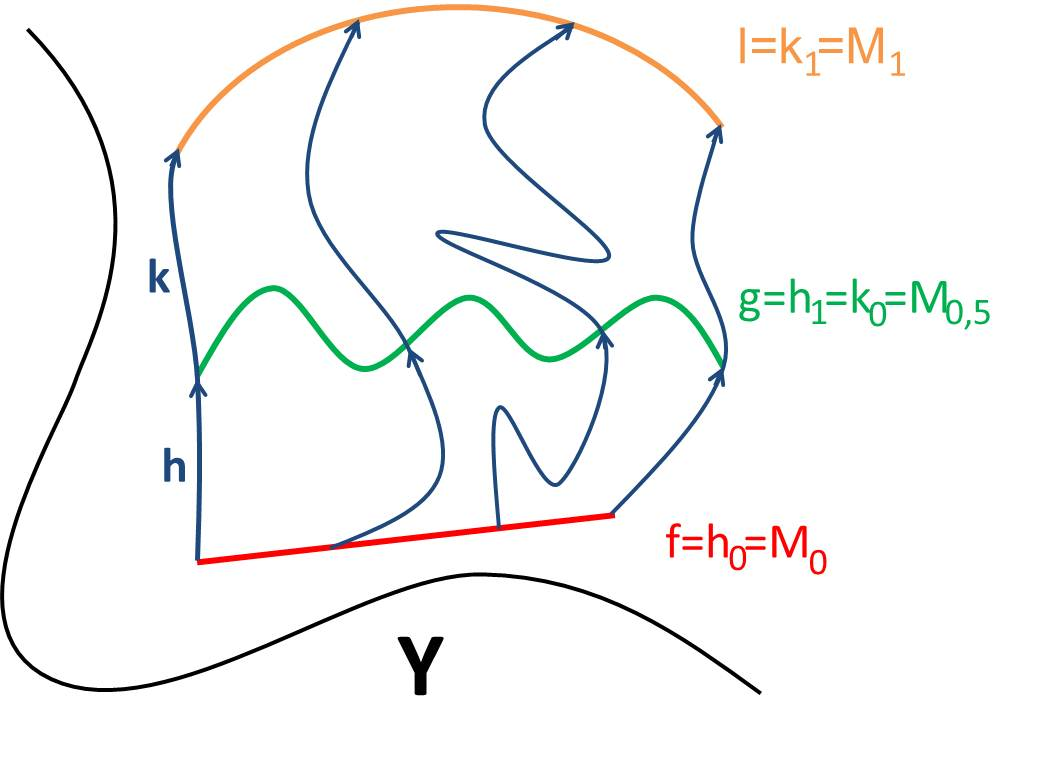
\includegraphics[width=0.8\textwidth]{images/Homotopie_Transitivitaet.jpg}
\caption{Transitivität der Relation "homotop sein"}
\end{figure}

\begin{remark}
Die Äquivalenzrelation "Homotopie von Abbildungen" liefert also eine Partition von $C(X,Y)$ in Äquivalenzklassen. Diese heißen Homotopieklassen und die \underline{Menge aller Homotopieklassen} \underline{stetiger Abbildungen} \underline{von $X$ nach $Y$} wird mit $[X,Y]$ bezeichnet.
\begin{figure}[h]
\centering
%\includegraphics[width=0.8\textwidth]{images/Äquivalenzklassen.jpg}
\caption{Äquivalenzklassen $[X,Y]$ von $C(X,Y)$}
\end{figure}
\end{remark}

\begin{remark}
$C(X,Y)$ ist im Allgemeinen \underline{\underline{viel}} schwieriger zu verstehen als $[X,Y]$!
\end{remark}

\begin{example}
Je zwei stetige Abbildungen $f,g \colon X \rightarrow \R^n$ sind homotop! Denn $H(x,t):= (1-t) f(x) + t \cdot g(x)$ liefert eine Homotopie von $f$ nach $g$:
\begin{figure}[h]
\centering
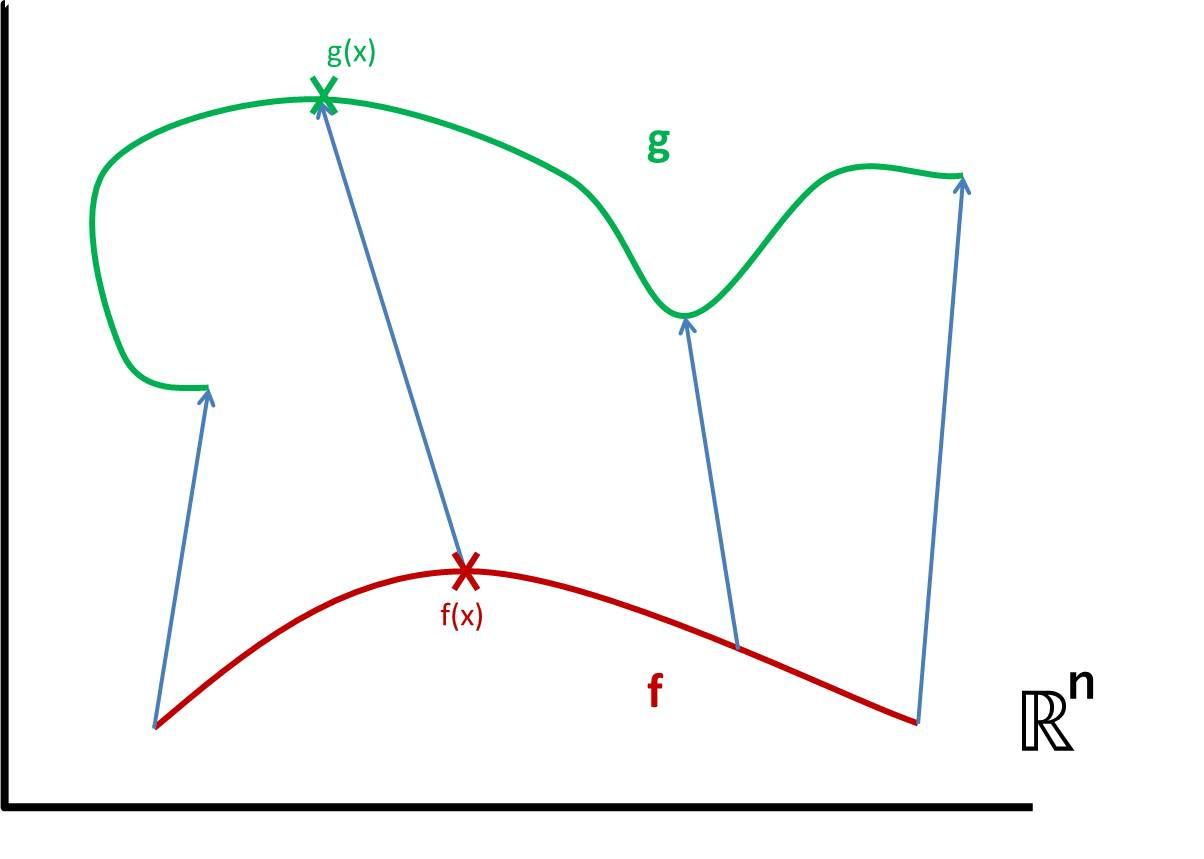
\includegraphics[width=0.8\textwidth]{images/R_n_immer_homotop.jpg}
\end{figure} 
\end{example}

%\begin{Kasten}
\begin{Kasten}{Nullhomotopie}
Eine stetige Abbildung $f \colon X \rightarrow Y$ heißt \underline{nullhomotop}, falls sie homotop zu einer konstanten Abbildung ist.
%\end{Kasten}
\end{Kasten}

\begin{figure}[h]
\centering
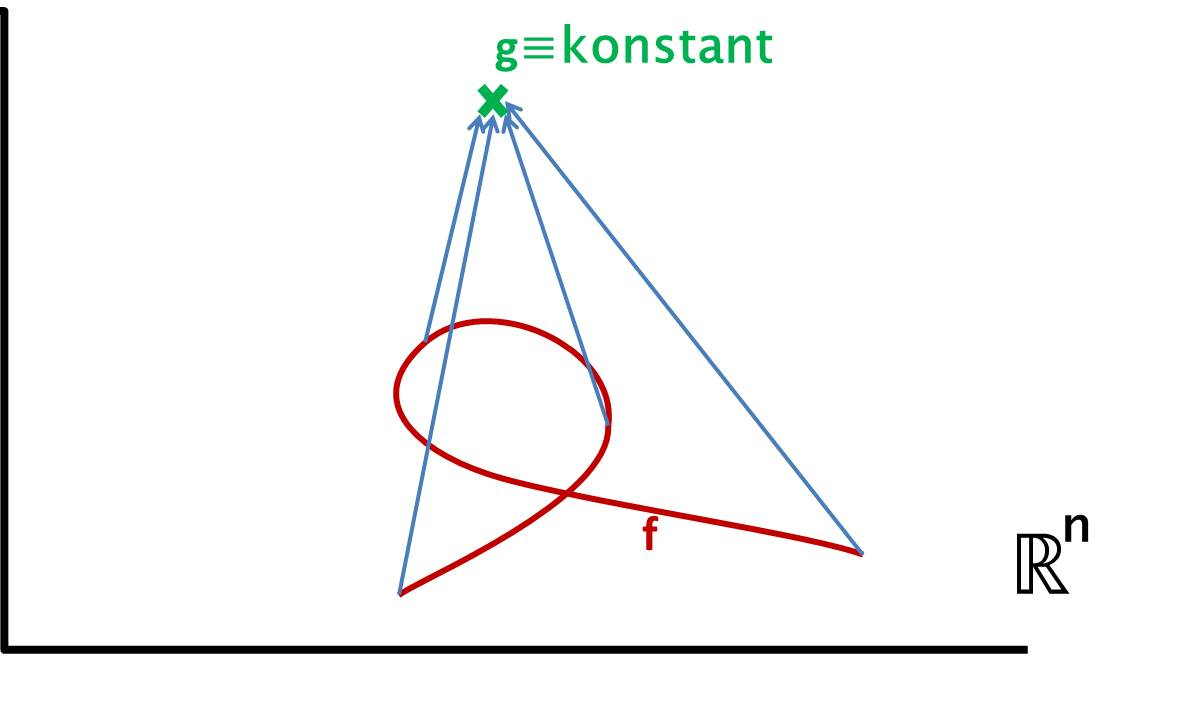
\includegraphics[width=0.8\textwidth]{images/Nullhomotopie.jpg}
\caption{f ist nullhomotop}
\end{figure}

\begin{corollary}
Jede stetige Abbildung $f \colon X \rightarrow \R^n$ ist nullhomotop, d.h. für jeden topologischen Raum $X$ besteht $[X, \R^n]$, $n$ beliebig, nur aus einem Punkt!
\end{corollary}

\begin{example}
Jeder \underline{geschlossene Weg im $\R^2$}, d.h. jede stetige Abbildung $f \colon [0,1] \rightarrow \R^2$ mit $f(0) = f(1)$ ist nullhomotop.
$\bigl[[0,1], \R^2\bigr]$ + gleicher Anfangs- und Endpunkt besteht nur aus einem Punkt, zum Beispiel der Äquivalenzklasse der konstanten Kurve $t \mapsto (1,0)$.

\begin{figure}[h]
\centering
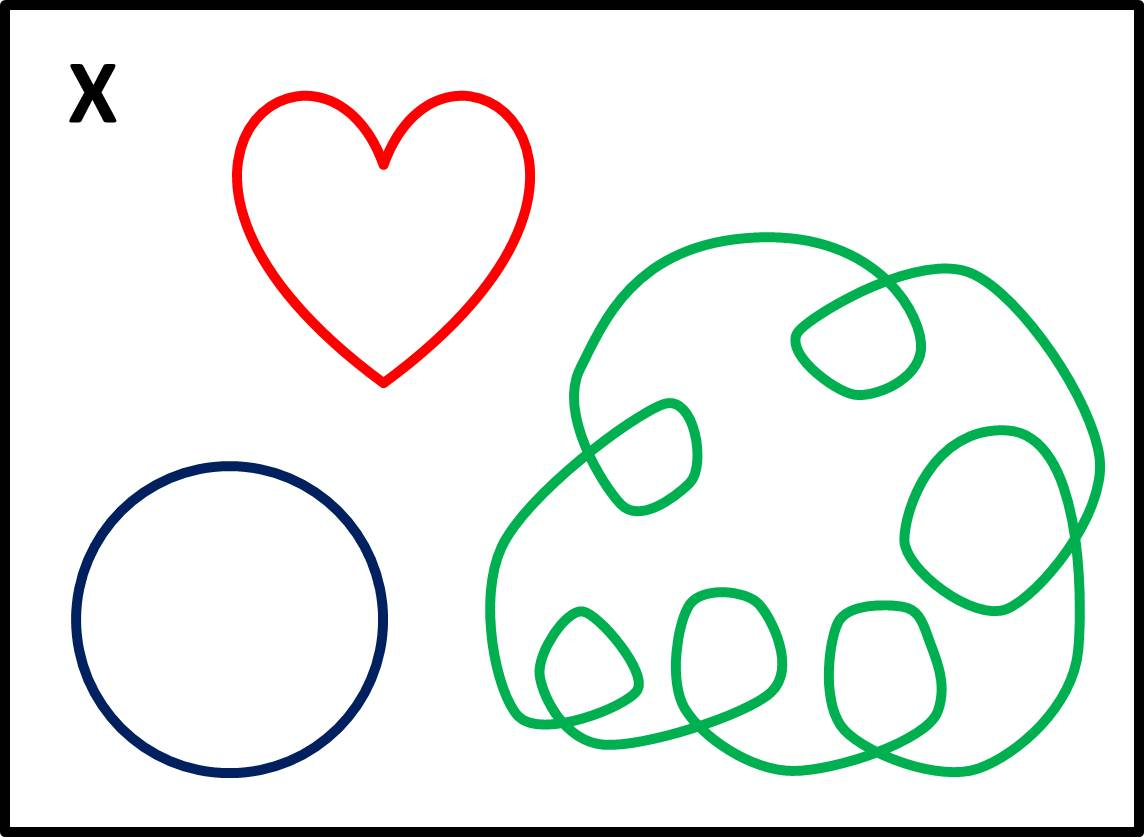
\includegraphics[width=0.8\textwidth]{images/Geschlossene_Wege.jpg}
\caption{Geschlossene Wege in $\R^n$}
\end{figure}

Interpretiere einen geschlossenen Weg im $\R^2$ auch als stetige Abbildung von $S^1 := \{ x \in \R^2 \mid \text{ } ||x|| = 1\}$ in $\R^2$, so gilt also $[S^1, \R^2]$ ist einelementig.
\newline
\underline{Aber} $[S^1, \R^2 \backslash \{0\}]$ ist nichttrivial! (TODO: BILD)
\end{example}

\begin{figure}[h]
\centering
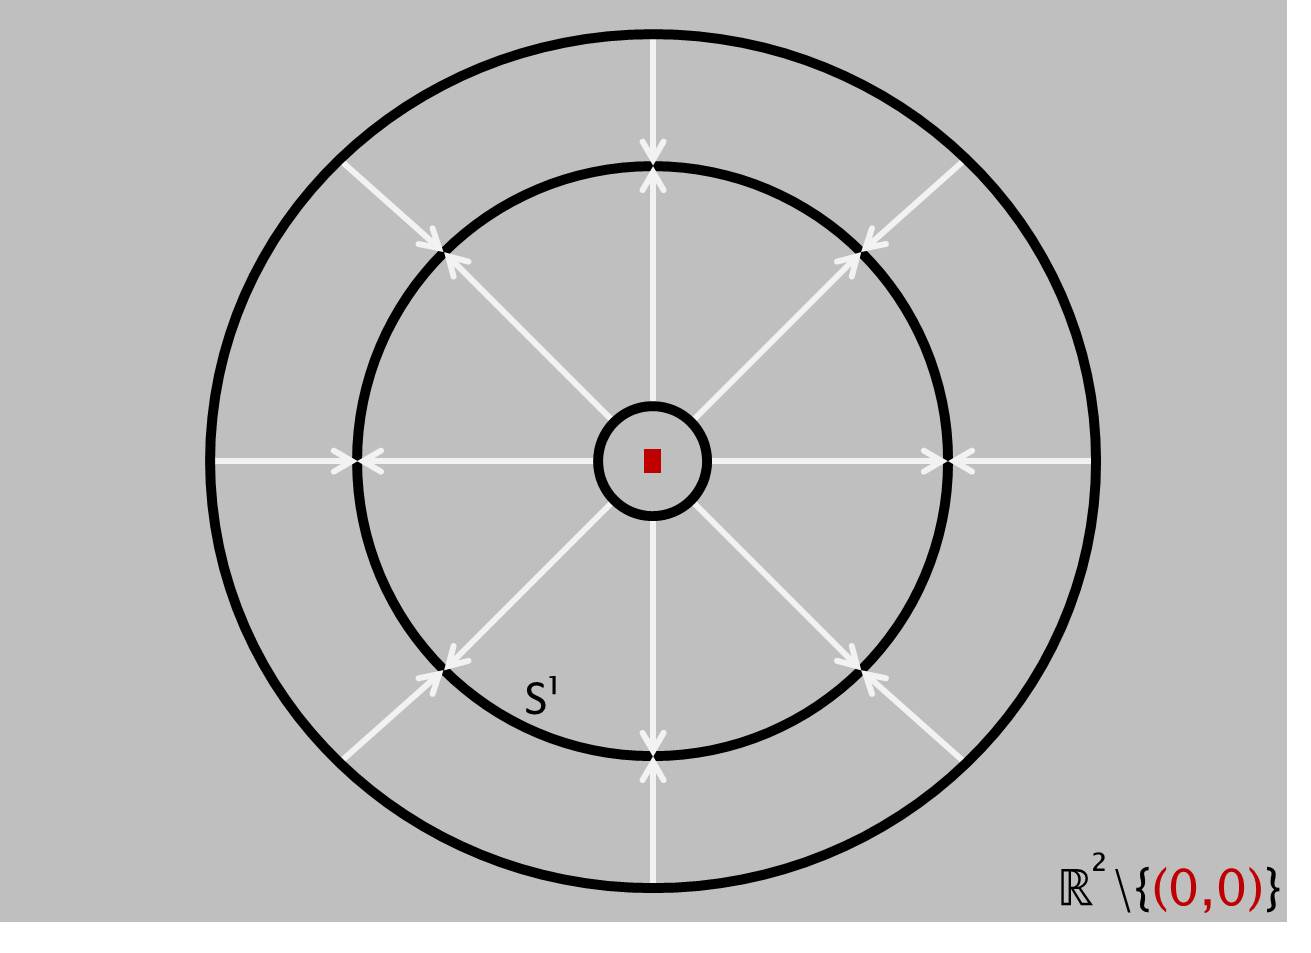
\includegraphics[width=0.8\textwidth]{images/S1_und_R2_ohne_0.jpg}
\caption{$[S^1,\R^2\setminus\{(0,0)\}]\text{ "=" }[S^1,S^1]$}
\end{figure}

%\begin{Kasten}
\begin{Kasten}{Teilraumtopologie}
Es sei $(X, \OO)$ topologischer Raum und $A \subset X$. Die auf $A$ durch
$$\OO \Big |_{A} := \{U \cap A \mid U \in \OO \}$$
induzierte Topologie heißt \underline{Teilraumtopologie} und der dadurch gegebene topologische Raum $(A, \OO \Big |_{A})$ heißt \underline{Teilraum} von $(X, \OO)$.
%\end{Kasten}
\end{Kasten}

\begin{remark}
$B \subset A$ ist also genau dann \underline{offen \underline{in $A$}}, wenn $B$ der Schnitt einer \underline{in $X$} offenen Menge mit $A$ ist.
\end{remark}

\begin{example}
$X = \R^2, A = S^1 = \{ x \in \R^2 \mid \text{ } ||x|| = 1\}$ 
\newline
\begin{figure}[h]
\centering
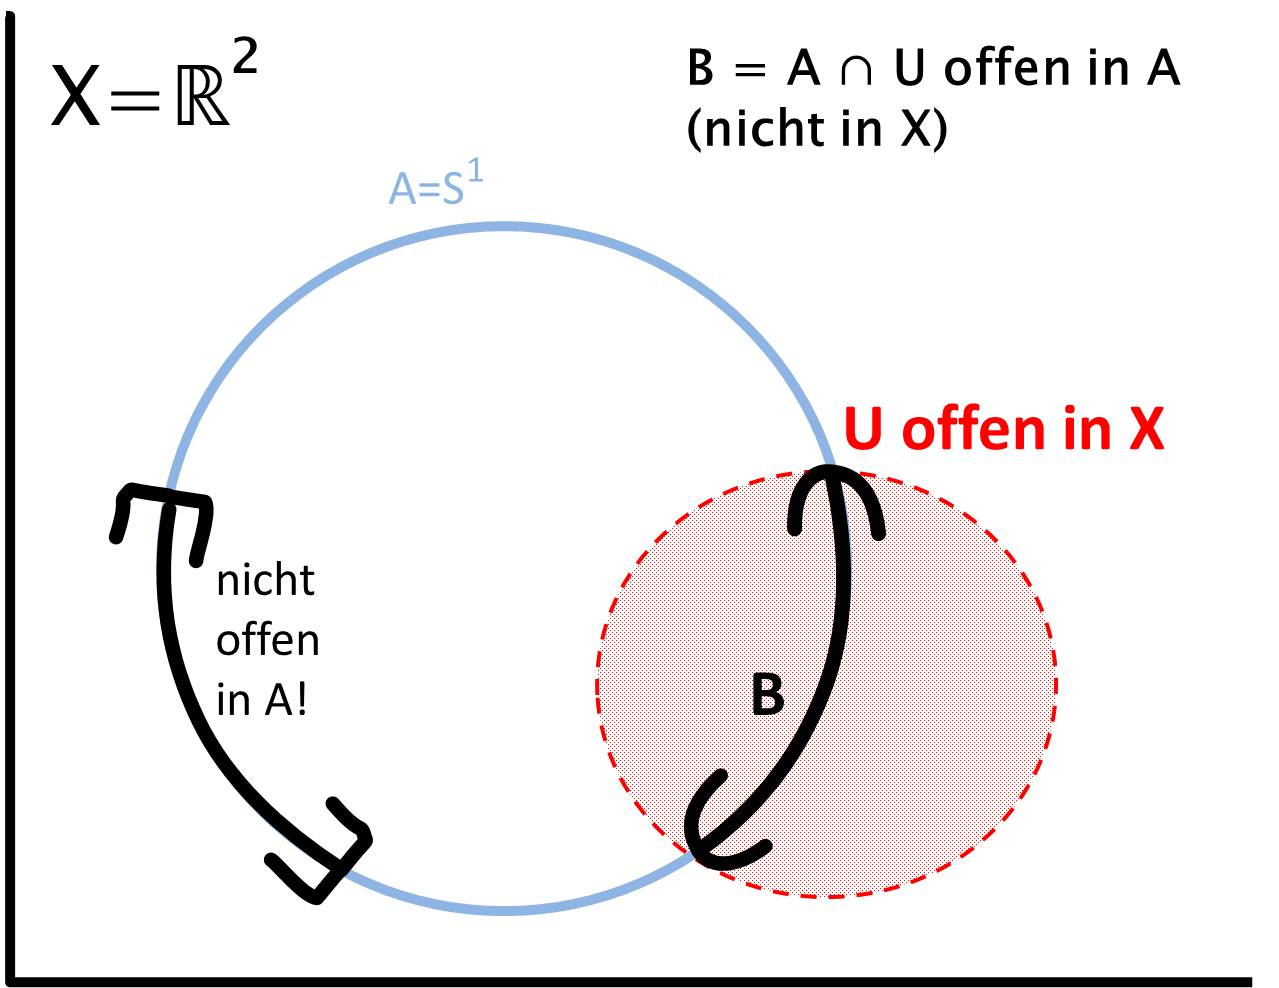
\includegraphics[width=0.8\textwidth]{images/Teilraumtopologie.jpg}
\end{figure}
\newline
\underline{Achtung:} $B$ ist \underline{\underline{nicht}} offen in $\R^2$!
\end{example}

\section{Grundlagen der allgemeinen Topologie}
\begin{example}[Beispiele topologischer Räume]
	\begin{enumerate}[(1)]
		\item $X, \OO := \{X, \emptyset\}$ \underline{`triviale Topologie'}
		\item $X, \OO := \mathcal{P}(X)$ \underline{`diskrete Topologie'}
		\item Metrische Räume, siehe unten
		\item $X:= \{a,b,c,d\} \Rightarrow \OO := \left\{X, \emptyset, \{a\}, \{b\}, \{a,c\}, \{a,b,c\}, \{a,b\} \right \}$ definiert eine Topologie auf $X$, aber $\OO^\prime:= \left \{ X, \emptyset, \{a,c,d\}, \{b,d\} \right \}$ nicht!
		\item $X := \R, \OO := \{O \mid \text{O ist Vereinigung von Intervallen } (a,b) \text{ mit } a,b \in \R\}$. $\Rightarrow (X, \OO) \text{ ist topologischer Raum}$, und $\OO$ heißt \underline{Standard-Topologie}.
		\item $X:= \R, \tilde{\OO} := \{O \mid O = \R \backslash E, E \subset \R \text{ endlich}\} \cup \{\emptyset\}$ ist auch eine Topologie auf $\R$, die so genannte $\mathcal{T}_1$-Topologie.
	\end{enumerate}
\end{example}

%\begin{Kasten}
\begin{Kasten}{Abgeschlossenheit}
	$A \subset X, X$ topologischer Raum, heißt \underline{abgeschlossen} $:\Leftrightarrow X \backslash A \text{ ist offen}$.
%\end{Kasten}
\end{Kasten}

\begin{remark}
	Beliebige Durchschnitte abgeschlossener Mengen sind abgeschlossen, ebenso endliche Vereinigungen und genauso $X$ und $\emptyset$.
\end{remark}

\begin{example}
	In einem diskreten topologischen Raum sind \underline{alle Teilmengen} abgeschlossen, in $\R_{\mathcal{T}_1}$\footnote{$\R$ mit $\mathcal{T}_1$-Topologie} alle endlichen Teilmengen und $X, \emptyset$.
\end{example}

%\begin{Kasten}
\begin{Kasten}{Umgebung}
	Ist $X$ topologischer Raum und $x \in X$, so heißt jede \underline{offene} Teilmenge $O \subset X$ mit $x \in O$ eine \underline{Umgebung} von $x$.
%\end{Kasten}
\end{Kasten}

\begin{remark}
	Umgebungen sind per definitionem offen! (TODO: BILD)
\end{remark}

\begin{remark}
	Jede offene Teilmenge von $\R_{Standard}$ ist eine Vereinigung disjunkter offener Intervalle, doch abgeschlossene Teilmengen von $\R$ sind keinesfalls immer Vereinigungen abgeschlossener Intervalle!
\end{remark}

\begin{example}[Die \underline{Cantor-Menge} $\mathcal{C}:= \left \{ x \in \R \mid x = \sum\limits_{k=1}^{\infty}{\frac{a_k}{3^k}}, a_k \in \{0,2\} \right \}$]
	$\Rightarrow$ $\mathcal{C}$ ist abgeschlossen in $\R$, enthält überabzählbar viele Elemente und hat `Hausdorff-Dimension' $\frac{\ln 2}{\ln 3} \approx 0,6 \ldots$
\end{example}

\begin{figure}[h]
\centering
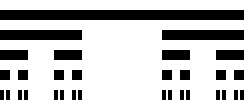
\includegraphics[width=0.8\textwidth]{images/Cantormenge_5te_Iteration.jpg}
\end{figure}

%\begin{Kasten}
\begin{Kasten}{Basis}
	Ist $(X, \OO)$ topologischer Raum mit $\mathcal{B} \subset \OO$, so heißt $\mathcal{B}$ \underline{Basis der Topologie} $:\Leftrightarrow$ Jede (nichtleere) offene Menge ist Vereinigung von Mengen aus $\mathcal{B}$.
%\end{Kasten}
\end{Kasten}

\begin{example}
	\begin{enumerate}[(1)]
		\item Die offenen Intervalle bilden eine Basis der Standard-Topologie von $\R$.
		\item Sämtliche offenen\footnote{bezüglich der euklidischen Metrik} Kreisscheiben 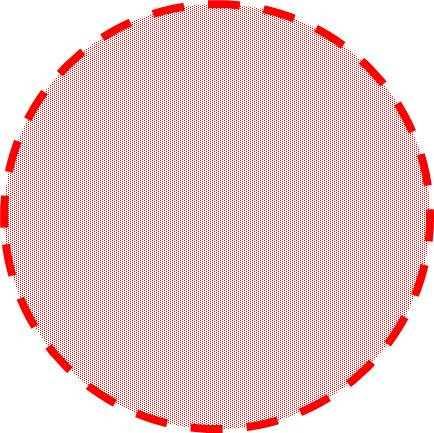
\includegraphics[scale=0.07]{images/offener_Kreis.jpg} und auch sämtliche offenen Quadrate 
\includegraphics[scale=0.07]{images/offenes_Quadrat.jpg} bilden Basen ein und derselben Topologie auf $\R^2$.
	\end{enumerate}
\end{example}

\begin{remark}
	$\bullet$ $\mathcal{B} \subset \OO$ ist Basis der Topologie von $X$ $\Leftrightarrow \forall O \in \OO \forall x \in O \exists B \in \mathcal{B} \colon x \in B \subset O$.
	\newline
	$\bullet$ $\mathcal{B} \subset \mathcal{P}(X)$ bildet die Bais \underline{einer} Topologie auf $X$ $\Leftrightarrow$ $X$ ist Vereinigung von Mengen aus $\mathcal{B}$ und der Schnitt je zweier Mengen aus $\mathcal{B}$ ist eine Vereinigung von Mengen aus $\mathcal{B}$.
	\newline
	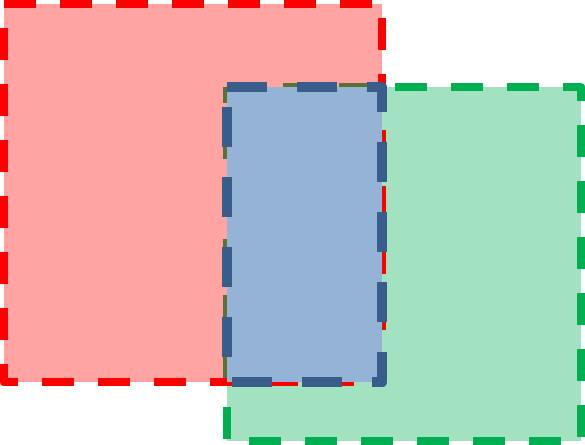
\includegraphics[scale=0.3]{images/Quadrate_Schnitt.jpg}\qquad
	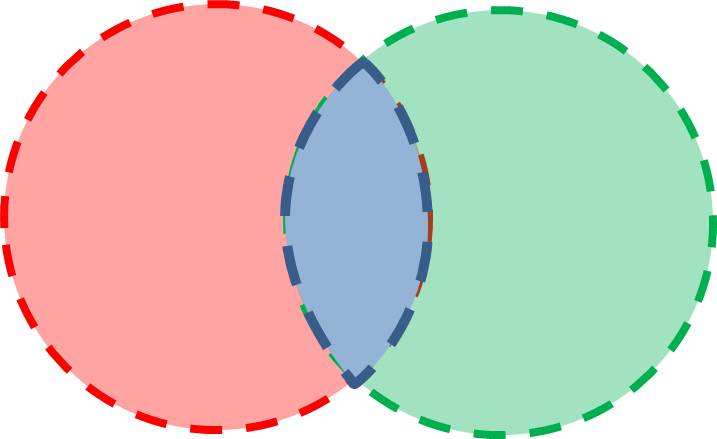
\includegraphics[scale=0.3]{images/Kreis_Schnitt.jpg}
\end{remark}

%\begin{Kasten}
\begin{Kasten}{Feiner und gröber}
	Sind $\OO_1$ und $\OO_2$ Topologien auf $X$ und $\OO_1 \subset \OO_2$, so heißt $\OO_2$ \underline{feiner} als $\OO_1$ und $\OO_1$ \underline{gröber} als $\OO_2$.
%\end{Kasten}
\end{Kasten}

\begin{example}
	$\bullet$ Die triviale Topologie ist die gröbste Topologie auf $X$, die diskrete Topologie die feinste.
	\newline
	$\bullet$ Die Standard-Topologie auf $\R$ ist feiner als die $\mathcal{T}_1$-Topologie.
\end{example}

\paragraph{Mehr zu metrischen Räumen}

%\begin{Kasten}
\begin{Kasten}{$\epsilon$-Ball, Sphäre}
	Für einen metrischen Raum $(X,d)$ und $\epsilon > 0$ sei für $p \in X$
	\begin{itemize}
		\item $B_\epsilon(p):=\{x \in C \mid d(p,x) < \epsilon \}$ der \underline{offene $\epsilon$-Ball um $p$}
		\item $D_\epsilon(p):=\{x \in C \mid d(p,x) \leq \epsilon \}$ der \underline{abgeschlossene $\epsilon$-Ball um $p$}
		\item $S_\epsilon(p):=\{x \in C \mid d(p,x) = \epsilon \}$ die \underline{ $\epsilon$-Sphäre} um $p$ (oder \underline{Sphäre vom Radius $\epsilon$})
	\end{itemize}
%\end{Kasten}
\end{Kasten}

%\begin{Kasten}
\begin{Kasten}{Metrischer Unterraum}
	Ist $(X,d)$ metrischer Raum und $A \subset X$, so heißt der metrische Raum $(A, d \big |_{A \times A})$ \underline{(metrischer) Unterraum von $X$}.
%\end{Kasten}
\end{Kasten}

\begin{example}
	Für $X=\R_{Eukl.}^{n}$ sind $B_1(0), D_1(0) =: D^n$ und $S^{n-1}:=S_1(0)$ metrische Unterräume und heißen auch offener bzw. abgeschlossener Einheitsball bzw. $(n-1)$-Sphäre.
	\newline
	(TODO: BILD)
\end{example}

%\begin{Kasten}
\begin{Kasten}{Beschränktheit, Durchmesser}
	$A \subset (X,d)$ heißt \underline{beschränkt} \newline $:\Leftrightarrow \exists 0 < \rho \in \R \colon d(x,y) < \rho  \text{   } \forall x,y \in A$
	\newline
	(TODO: BILD)
	\newline
	Das Infimum, diam $A$, dieser $\rho$ heißt dann \underline{Durchmesser von $A$}.
%\end{Kasten}
\end{Kasten}

\begin{remark}
	In einem metrischen Raum $(X,d)$ bilden die offenen Bälle die Basis einer Topologie $\OO=\OO_d$ von $X$, diese heißt \underline{die von der Metrik induzierte Topologie}.
\end{remark}

\begin{remark}
	$A \subset (X,d)$ ist \underline{offen}
	\newline
	$\Leftrightarrow \forall p \in A \exists \text{ ein offener Ball } B_\epsilon(p) \text{ um } p \text{ mit } B_\epsilon(p) \subset A$
	\newline
	(TODO: BILD)
\end{remark}

%\begin{Kasten}
\begin{Kasten}{Abstand}
	$(X,d)$ sei metrischer Raum und $A \subset X, p \in X$.
	$$d(p,A) := dist(p,A):= \inf \{d(p,a) \mid a\in A \}$$
	heißt \underline{Abstand von $p$ und $A$}.
%\end{Kasten}
\end{Kasten}

\paragraph{Erinnerung}
Ist $(X, \OO)$ topologischer Raum und $A \subset X$, so definiert
$\OO_A := \{ A \cap O \mid O \in \OO \}$ eine Topologie auf $A$, die
 \underline{Teilraumtopologie} der \underline{in A} offenen Mengen.
 
\begin{remark}
	\label{offenAbgeschlossen}
	Ist $A \subset X$ \underline{offen} \underline{\underline{in $X$}}, so ist auch jede in $A$ offene Menge offen in $X$, und abgeschlossene\footnote{in $A$} Teilmengen einer in $X$ abgeschlossenen Menge $A$ sind auch abgeschlossen in $X$.
	
	(TODO:BILD)
	\newline
	Aber abgeschlossene Mengen $B$ in $A \subset X$ sind für beliebiges $A$ im Allgemeinen nicht abgeschlossen in $X$.
\end{remark}

\begin{example}[Beispiel zu Bemerkung~\ref{offenAbgeschlossen}]
	$B := A := (a,b) \subset X := \R$
\end{example}

\begin{Kasten}{Innerer Punkt, äußerer Punkt, Randpunkt}
	Für $p \in A \subset X$, $X$ topologischer Raum, heißt $p$
	\newline
	\begin{enumerate}[(1)]
		\item \underline{innerer Punkt} von $A$, falls es eine in $A$ enthaltene Umgebung $U$ um $p$ gibt. (TODO:BILD)
		\item \underline{äußerer Punkt}, falls eine zu $p$ disjunkte Umgebung $V$ in $X$ existiert.
		\item \underline{Randpunkt von $A$}, falls jede Umgebung von $p$ nichtleeren Durchschnitt mit $A$ und $X \backslash A$ hat.
	\end{enumerate}
\end{Kasten}

\begin{Kasten}{Inneres}
	Für $A \subset X$ heißt die größte in $X$ offene und in $A$ enthaltene Teilmenge $\mathring A$ \underline{Inneres von $A$}.
\end{Kasten}

\begin{remark}
	$\mathring A$ ist die Menge aller inneren Punkte von $A$ und die Vereinigung aller in $X$ offenen Teilmengen von $A$, und $A \text{ ist offen } \Leftrightarrow A = \mathring A$
\end{remark}

\begin{example}
	$\mathring {\R \backslash \Q} = \mathring \Q = \emptyset$
\end{example}

\begin{Kasten}{Abschluss}
	Der \underline{Abschluss} $\bar{A}$ von $A$ ist $X \backslash \left ( \mathring {(X \backslash A} ) \right )$.
\end{Kasten}

\begin{Kasten}{Rand}
	Der \underline{Rand} $\partial A$ von $A$ ist $\partial A := \bar{A} \backslash \mathring A$, d.h. Rand $A$ = \{ Randpunkte von A \}.
\end{Kasten}

(TODO:Exkurs zu `Randbildung (topologisch) und Ableitung (analytisch) sind dual zueinander')

\begin{Kasten}{Stetigkeit}
	$f \colon X \rightarrow Y$ ist stetig $:\Leftrightarrow \forall$ offenen Mengen in $Y$ ist das Urbild unter $f$ offene Menge in $X$.
\end{Kasten}

\begin{example}
	\begin{itemize}
		\item $f \colon X \rightarrow Y$ ist stetig $\Leftrightarrow$ Urbilder abgeschlossener Mengen sind abgeschlossen.
		\item Sind $\OO_1$ und $\OO_2$ Topologien auf $X$, so ist die Identität $\text{id} \colon (X,\OO_1) \rightarrow (X,\OO_2)$ stetig $\Leftrightarrow \OO_2 \subset \OO_1$.
		\item Für $A \subset X$ ist die Teilraumtopologie $\OO_A = \OO \big |_A$ die gröbste Topologie, bezüglich der die Inklusion $i \colon A \hookrightarrow X, a \mapsto a$ stetig ist.
	\end{itemize}
\end{example}

\begin{Kasten}{Stetigkeit} %spacings stimmen nicht ganz (TODO)
	$f \colon X \rightarrow Y$ ist stetig in $x \in X$
	$:\Leftrightarrow \forall \text{ Umgebungen } V \text{ von } f(x) \exists \text{ Umgebung } U \text{ von } x \text{ und } f(U) \subset V$
	\newline
	(TODO:BILD)
\end{Kasten}

\begin{remark}
	$f \colon X \rightarrow Y$ ist stetig $\Leftrightarrow$ $f$ ist stetig in jedem Punkt $x \in X$.
\end{remark}

\begin{example}
	Eine Abbildung $f \colon X \rightarrow Y$ zwischen \underline{metrischen} Räumen ist bezüglich der von den Metriken induzierten Topologien stetig in $x \in X$ genau dann, wenn für jeden offenen Ball $B$ um $f(x)$ ein offener Ball um $x$ existiert, der unter $f$ in $B$ abgebildet wird. (Und ferner stetig in $x \in X$ genau dann, wenn für alle $\epsilon > 0$ ein $\delta > 0$ existiert, so dass für alle $x^\prime \in X$ mit $d_X(x,x^\prime) < \delta$ auch $d_Y \left( f(x), f(x^\prime) \right) < \epsilon$ folgt.) 
\end{example}

\begin{Kasten}{Isometrische Einbettung, Isometrie}
	Sind $X,Y$ metrische Räume, so heißt eine Abbildung $f \colon X \rightarrow Y$ \underline{isometrische Einbettung}
	\newline	
	 $: \Leftrightarrow \forall x, x^\prime \in X$ gilt $d_Y \left ( f(x), f(x^\prime) \right ) = d_X (x, x^\prime)$.
	\newline
	Eine isometrische Einbettung ist immer injektiv.
	\newline
	Ist $f$ zusätzlich \underline{bijektiv}, so heißt $f$ \underline{\underline{Isometrie}}. 
\end{Kasten}

\begin{Kasten}{Homöomorphismus}
	Eine invertierbare Abbildung $f \colon X \rightarrow Y$ topologischer Räume heißt \underline{Homöomorphismus}, falls $f$ und $f^{-1}$ stetig sind.
\end{Kasten}

\begin{example}
	\begin{itemize}
		\item $f \colon [0,1) \rightarrow S^1 \subset \C \hat{=} \R^2, t \mapsto e^{2 \pi i t} (= \cos {2 \pi t}, \sin {2 \pi t})$ ist stetig, injektiv, aber \underline{kein} Homöomorphismus!
		\newline
		(TODO:BILD)
		\item $id_X \colon X \rightarrow X$ ist immer ein Homöomorphismus, Kompositionen von Homöomorphismen ebenfalls.
	\end{itemize}
\end{example}

\begin{remark}
	`Homöomorph sein' ist eine Äquivalenzrelation für topologische Räume.
\end{remark}

\begin{Kasten}{homöomorph}
	Zwei topologische Räume $X$ und $Y$ heißen \underline{homöomorph} oder \underline{vom gleichen Homöomorphietyp}, in Zeichen $X \cong Y$, falls es einen Homöomorphismus $f \colon X \rightarrow Y$ gibt.
\end{Kasten}

\begin{remark}
	Homöomorphismen erhalten sämtliche topologischen Strukturen:
	\begin{itemize}
		\item Ist $f \colon X \rightarrow Y$ Homöomorphismus, so ist $U \subset X$ offen $\Leftrightarrow f(U)$ offen in $Y$.
		\item $A \subset X$ ist abgeschlossen $\Leftrightarrow f(A)$ ist abgeschlossen in $Y$.
		\item $f(\bar{A}) = \overline{f(A)}, f(\mathring A) = \mathring{\left(f(A)\right)}$.
		\item $U$ ist Umgebung von $x \in X$ $\Leftrightarrow f(U)$ ist Umgebung von $f(x)$.
	\end{itemize}
\end{remark}

\begin{example}
	\begin{itemize}
		\item Jede Isometrie zwischen metrischen Räumen ist ein Homöomorphismus.
		\item $[0,1] \cong [a,b] \forall a < b \in \R$
		\item $(0,1) \cong (a,b) \cong \R \forall a < b \in \R$
	\end{itemize}
\end{example}

\begin{example}{Stereographische Projektion}\newline
	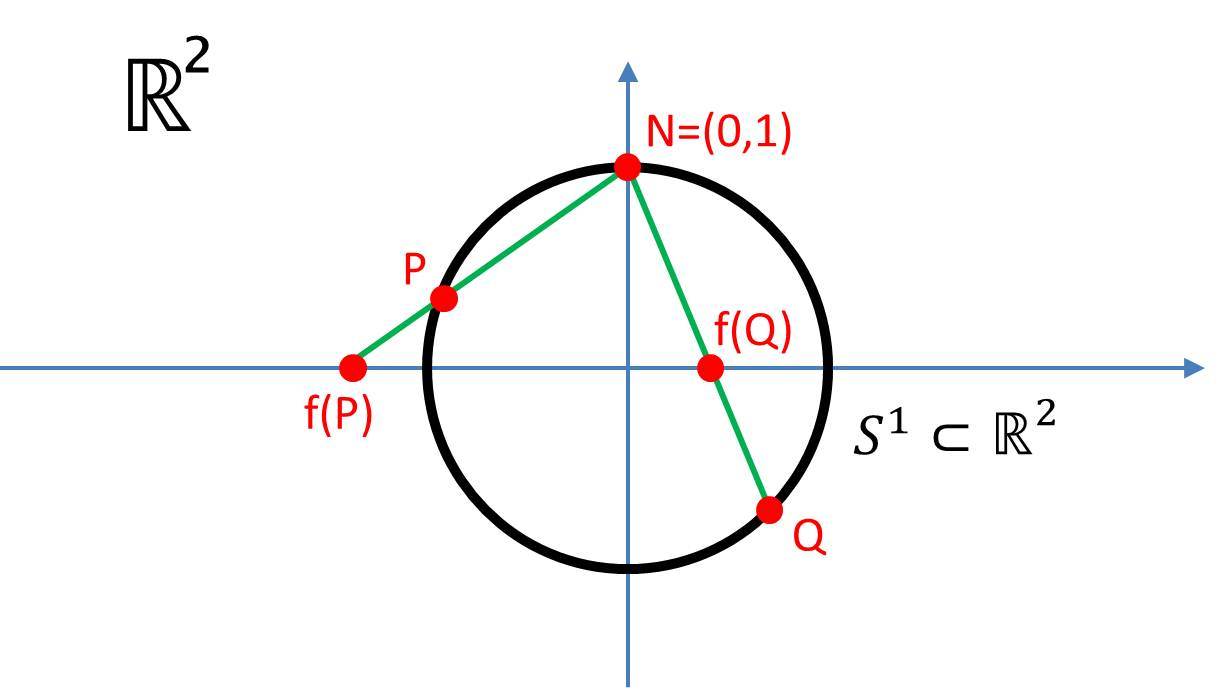
\includegraphics[scale=0.4]{images/Stereographie_S1_R1.jpg}
	\newline
	Die stereographische Projektion ist ein Homöomorphismus von $S^n \backslash \{N\}, N := (0, \ldots, 0, 1) \in \R^{n+1}$, gegeben wie folgt:
	\newline
	Der Schnitt der Geraden im $\R^{n+1}$ durch $N$ und $x \in S^n \backslash \{N\}$ mit der Hyperebene $\R^n=\{x \in \R^{n+1} \mid x_{n+1} = 0 \}$, $f(x)$, ist gegeben durch $x = (x_1, \ldots, x_{n+1}) \mapsto (\frac{x_1}{1-x_{n+1}}, \frac{x_2}{1-x_{n+1}}, \ldots, \frac{x_n}{1-x_{n+1}}) =: f(x)$ mit Umkehrabbildung $y = (y_1, \ldots, y_n) \mapsto (\frac{2 y_1}{||y||^2+1}, \ldots, \frac{2 y_n}{||y||^2+1},\frac{||y||^2-1}{||y||^2+1})$.
\end{example}

\begin{Kasten}{Einbettung}
	$f \colon X \rightarrow Y$ stetig heißt \underline{Einbettung} $:\Leftrightarrow X \overset{f}{\rightarrow}f(X) \subset Y$ Homöomorphismus.
\end{Kasten}

\begin{example}
	\begin{itemize}
		\item Für $A \subset X$ ist die Inklusion $\iota \colon A \hookrightarrow X$
	\end{itemize}
\end{example}
TODO: Vorlesung vom Donnerstag

\section{Trennungeigenschaften}
\begin{Kasten}{$T_1$-Raum}
Ein topologischer Raum $X$ heißt \underline{$T_1$-Raum} bzw. \underline{erfüllt das erste Trennungsaxiom} $:\Leftrightarrow$ Für je zwei verschiedene Punkte von $X$ existiert für jeden dieser Punkte eine Umgebung in $X$, die den anderen nicht enthält. (TODO:Bild)
\newline
$\forall x \neq y \in X \exists U = U_X \colon y \notin U_X$ 
\end{Kasten}

\begin{Kasten}{$T_2$-Raum}
	$X$ heißt \underline{Hausdorff}- oder \underline{$T_2$-Raum} bzw. \underline{erfüllt das zweite Trennungsaxiom} $:\Leftrightarrow$ Je zwei verschiedene Punkte in $X$ besitzen disjunkte Umgebungen.
	\newline
	$\forall x \neq y \in X \exists U_x \ni x, U_y \ni y$ mit $U_x \cap U_y = \emptyset$
	(TODO:Bild)
\end{Kasten}

\begin{example}
	Jeder metrische Raum ist Hausdorff-Raum.
\end{example}

\begin{remark}
Hausdorff-Räume sind z.B. deshalb wichtig, weil Grenzwerte dort eindeutig sind!
\end{remark}

\begin{definition}
Ist $(x_n)_{n \in \N}$ eine Folge von Punkten in einem topologischen Raum $X$, so heißt $x \in X$ \underline{Grenzwert} der Folge $(x_n)$ genau dann, wenn zu jeder Umgebung $U$ von $x$ $N \in \N$ existiert mit $x_n \in U \forall n \geq N$. 
\newline
(TODO:Bild)
\end{definition}

\begin{example}
In einem Hausdorff-Raum hat jede Folge höchstens einen Grenzwert.
\end{example}

\begin{remark}
Hausdorff-Räume sind auch $T_1$-Räume, aber:
\end{remark}

\begin{example}
	In $X=\R_{\mathcal{T}_1}$ ist jeder Punkt abgeschlossen ($\Rightarrow T_1$), doch je zwei nichtleere offene Mengen schneiden sich - $X$ ist damit nicht $T_2$!
	%newline
	\underline{"Schlimmer":} In $\R_{\mathcal{T}_1}$ ist \underline{jeder} Punkt Grenzwert der Folge $x_n = n$!
	Denn eine Umgebung eines Punktes in $\R_{\mathcal{T}_1}$ hat die Form $U = \R \backslash \{x_1, \ldots, x_M\}$ mit $x_1 < \ldots < x_M$. Dann gilt aber $x_n = n \forall n > x_M$
\end{example}

\section{Abzählbarkeitsaxiome}
\begin{Kasten}{Umgebungsbasis}
	Ist $X$ topologischer Raum und $x \in X$, so ist eine \underline{Umgebungsbasis} oder \underline{Basis von $X$} \underline{\underline{in $x$}} eine Familie von Umgebungen von $x$, sodass \underline{jede} Umgebung von $x$ eine Umgebung aus der Familie enthält.
\end{Kasten}

\begin{example}
	Ist $B$ Basis der Topologie eines Raumes $X$, so ist für jedes $x \in X$ $\{U \in B \mid x \in U\}$ eine Basis von $X$ \underline{\underline{in $x$}}
\end{example}

\begin{example}
	In einem \underline{metrischen} Raum $X$ sind folgende Mengen von Bällen Basen von $X$ in $x \in X$:
	\begin{itemize}
		\item alle offenen Bälle mit Zentrum $x$
		\item alle offenen Bälle mit Zentrum $x$ mit rationalen Radii
	\end{itemize}
\end{example}

\begin{example}
	Ist $X$ mit der diskreten bzw. trivialen Topologie versehen, so ist die `kleinste' Basis in $x \in X$ gegeben durch $\left\{\{x\}\right\}$ bzw. $\{X\}$.
\end{example}

\begin{Kasten}{Abzählbarkeitsaxiome, Separabilität}
	$X$ \underline{erfüllt das erste Abzählbarkeitsaxiom}
	$:\Leftrightarrow$ jeder Punkt $x \in X$ besitzt eine abzählbare Basis.
	\newline
	$X$ \underline{erfüllt das zweite Abzählbarkeitsaxiom}
	$:\Leftrightarrow$ $X$ selbst besitzt eine abzählbare Basis.
	\newline
	$X$ heißt \underline{separabel} $\Leftrightarrow$ $X$ enthält eine abzählbare und dichte ($\bar{A} = X$) Menge $A$.
\end{Kasten}
 
\begin{remark}
	Das zweite Abzählbarkeitsaxiom impliziert das erste, aber:
\end{remark} 

\begin{example}
	Überabzählbare diskrete Räume (wie $(\R, \OO_{diskret})$)!
\end{example}
 
\begin{remark}
	Jeder metrische Raum erfüllt das erste Abzählbarkeitsaxiom und jeder \underline{separable} metrische Raum auch das zweite.
\end{remark} 
 
\begin{example}
	$\R_{\mathcal{T}_1}$ erfüllt \underline{nicht} das erste Abzählbarkeitsaxiom, ist aber separabel - $\N$ ist dicht!
\end{example} 
 
\begin{example}
	Euklidische Räume und alle ihre Teilmengen erfüllen das 2. Abzählbarkeitsaxiom und sind separabel.
\end{example} 
 
Wozu das Ganze? 
\newline $\rightsquigarrow$ Funktionenräume
\newline $\rightsquigarrow$ Mannigfaltigkeiten
\newline $\rightsquigarrow$ \underline{Satz von Lindelöf:}
Jede offene Überdeckung eines Raumes, der das zweite Abzählbarkeitsaxiom erfüllt, enthält auch eine abzählbare \underline{Teilüberdeckung}.
 
\begin{Kasten}{Lokale Kompaktheit}
$X$ heißt \underline{\underline{lokal} kompakt} \newline $:\Leftrightarrow$ Jeder Punkt $x \in X$ besitzt eine Umgebung $U$, sodass $\overline{U}$ kompakt ist.
\end{Kasten} 

\begin{Kasten}{Lokale Endlichkeit}
	Eine Familie $\Gamma$ von Teilmengen eines topologischen Raumes $X$ heißt \underline{lokal endlich} $:\Leftrightarrow \forall x \in X \exists U = U(x) \colon A \cap U = \emptyset \forall A \in \Gamma$ bis auf endlich viele $A$. (TODO:Bild)
\end{Kasten}
 
\begin{Kasten}{Verfeinerung}
	$\Gamma, \Delta$ Überdeckungen von $X$. $\Delta$ heißt \underline{Verfeinerung} von $\Gamma$ \newline $:\Leftrightarrow \forall A \in \Delta \exists B \in \Gamma \colon A \subset B$.
\end{Kasten} 

\begin{Kasten}{Parakompaktheit}
	$X$ heißt \underline{parakompakt} $:\Leftrightarrow$ Jede offene Überdeckung besitzt eine lokal endliche offene Verfeinerung. 
\end{Kasten}

(TODO:Bild) \underline{\underline{Cut-off}}
 
\end{document}
